\section{Related Work}
\label{s:related-work}

Search Enginee Optimization (SEO) is encouraged by Seach Enginee companies like Google to improve the indexing and searching accuracy. SEO technology being used should follow the Google Policy. However, because imfluencing the search results has huge commerical incentives, some hackers designed Black Hat SEO which violate Google's policy. Cloaking is a representative of Black Hat SEO. Websites feed different information between Google and Users. In our study, we found that cloaking not only exists in SEO field but also Search Engiee Marketing (SEM). SEM is a term that exclusively to mean pay per click advertising, particularly in the commercial advertising and markerting communities which have a vested interest in thisnarrow defination. Advertisers pay Google to advertise one kind of advertisements. By cloaking, advertisers actually cheat Google and provide different kinds of advertisements, even maladvertising~\cite{Li:2012:KYE:2382196.2382267} and malicious attacks. 

\subsection{Cloaking Example}
As an example of cloaking in SEM, enter the term "essay writing" on Google on Feb 6, 2015 returned a set of search results and advertisements related to essay writing. (The appendix includes screenshots of this example.) For the second advertisement result in right side, the bold line circle the webstie (everlastinghelp.com) that is sending google 


\begin{figure}[t]
	\centering
	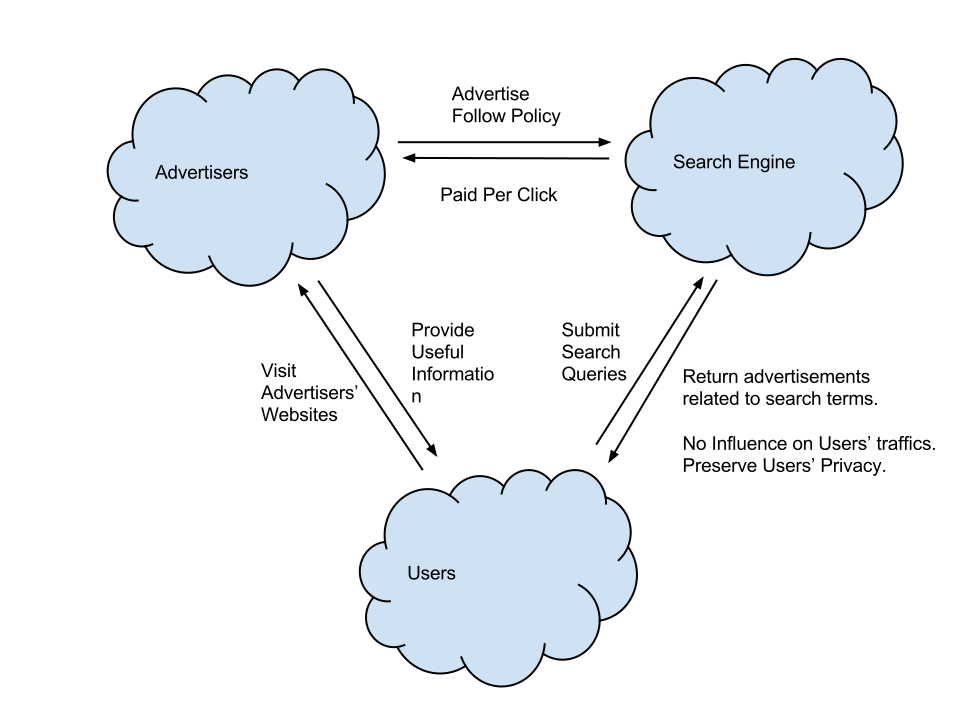
\includegraphics[width=.5\textwidth]{fig/three-parties}
	\label{fig:sem-model}
	\caption{Three-paries relationships in SEM}
\end{figure}

\subsection{Cloaking Detection}
Talk about cloaking detection related work here.
According to ~\cite{wang2011cloak}, they used the precision rate to measure the cloaking distribution on the search enginee hot terms. However, precision is highly depends on TRP and FPR. Using the precision to measure the distribution is fundamentally wrong method to do that. One of the right ways is using the TPR and FPR to measure the distribution. Another mistake they made is using constant numbers to measure time-based data without doing cross-validation. One way to do that is using the cross-validation or time-based adaptive parameter to solve this problem. 

Tree party relationships in SEM field. 
To better understanding the advantages of our crowdsourcing model, we briefly introduce the relationships in Search Enginee Markering (SEM). 

Traditional cloaking detection model only targets SEO field, our simhash based cloaking detection method could work both on SEO and SEM field. The main difference between the SEM and SEO is that every link in SEM is "pay per click". This indicates that  traiditional crawler will increase the advertisers payments by clicking the search result links and collecting data. If the cralwers first collect the landing page of the search result links then visit urls to collect data. The crawlers won't find the referal cloaking accoding to defination of referal cloaking. However, in our crowdsoucing model, the data we collected is from real users' clicks. Advertisers wouldn't pay extra money because of data collection. 
Model based on crowdsourcing could preserve the three party relationships between Users, Search Enginee Providers and Advertisers.



\subsection{Simhash}
Talk about simhash related work here. \\
Simhash~\cite{charikar2002similarity}  is a locality sensitive hash algorithm.
It is widely used by search engine to detect near duplicate of websites.


Show what simhash does and how they are used in the past.

Some embedded literal typeset code might 
look like the following :

{\tt \small
  \begin{verbatim}
  int wrap_fact(ClientData clientData,
  Tcl_Interp *interp,
  int argc, char *argv[) {
    int result;
    int arg0;
    if (argc != 2) {
      interp->result = ``wrong # args'';
      return TCL_ERROR;
    }
    arg0 = atoi(argv[1]);
    result = fact(arg0);
    sprintf(interp->result,``%d'',result);
    return TCL_OK;
  }
  \end{verbatim}
}

Now we're going to cite somebody.  Watch
for the cite tag.
Here it comes%~\cite{Chaum1981,Diffie1976}.
The tilde character (\~{})
in the source means a non-breaking space.
This way, your reference will
always be attached to the word that preceded it,
instead of going to the
next line.


\subsection{Simhash in Cloaking Detection}
Show the story here please!

1.what is the technical challege that we are addressing? compared to traditional
methods.

a. attacker could incrementally block inspector IP
b. crowdsourcing is cheap, compared to buying new IPs
c. crowdsourcing match user distribution and user habbit on web ~\cite{wang2011cloak}.

2. why we need simhash.
reduce volume of data, and collect enough information for cloaking detection.


3. what is user incentive?
build an extension to help user understand whether this website is
safe/compliant or tricking user by cloaking

user privacy is protected and can get better service.




